\chapter{Front-end}

Como falado no capítulo da arquitetura, a página é gerada no lado do servidor, então o que 
é retornado para cada rota é um HTML já pronto. Acredito que, para o meu caso, é mais 
performático fazer assim do que usar páginas com Javascript que fazem requisição para uma API REST.
Além disso, o desenvolvimento é mais rápido já que não é necessário codificar o front-end.
Para um projeto individual isto tem funcionado bem, mas claro que, para um projeto com
mais pessoas, seria melhor fazer uma API REST já teríamos um time para back-end e outro
para front-end.

De todo modo, no final da execução de uma rota, um dicionário Python é gerado, algo que 
poderia ser facilmente convertido para um JSON usando a função \texttt{dumps()} da 
biblioteca \texttt{json} do próprio Python. No caso desta aplicação, este dicionário é 
enviado para o template usando a função \texttt{render\_template()} da biblioteca Jinja2, 
que recebe o nome da página HTML com o template e um número qualquer de \textit{kwargs} (argumentos nomeados) 
que podem ter qualquer tipo serializável, incluindo dicionários.

Perceba que não há problema de acoplamento fazendo deste modo, pois não há código HTML sendo 
escrito dentro do backend. Como já dito, o que é passado para o Jinja é algo equivalente a JSON.
Transformar este backend em uma API REST não seria muito difícil.

Uma página template é um arquivo HTML com \textit{placeholders} que serão substituídos pelos 
\textit{kwargs} de mesmo nome. O Jinja2 tem estruturas de repetição para que um código HTML 
possa ser repetido usando valores da lista. E, no caso de dicionários e listas, é fácil acessar 
os valores. Neste projeto, para exibir a lista de frequência, o seguinte código é usado.

\lstinputlisting[label=cod:jinja-comm,title={Template de comunicação com o Jinja},caption={Template de comunicação com o Jinja},language=HTML]{code/jinja-comm.html}

É possível fazer operações e formatações simples no Jinja2. Já que a frequência 
é armazenada no banco como um inteiro de ponto fixo (como dito no capítulo de modelo de dados), 
foi criado o filtro "frequency3" para exibir o número corretamente. Um "filtro" no Jinja 
é apenas uma função que recebe e retorna
uma string. O filtro é chamado usando a sintaxe "\{\{variavel | funcao\}\}".


Note que caso a variável "isAdmin" seja definida, um botão de alterar a frequência aparece. Este
e outros botões de adição e edição são mostrados quando existe uma seção de usuário aberta para que o administrador
consiga editar um aeródromo.

No código do projeto, na pasta 'templates', é possível ver todos os templates usados.

\section{Imagens da Interface Gráfica}

\begin{figure}[ht]
    \begin{center}
    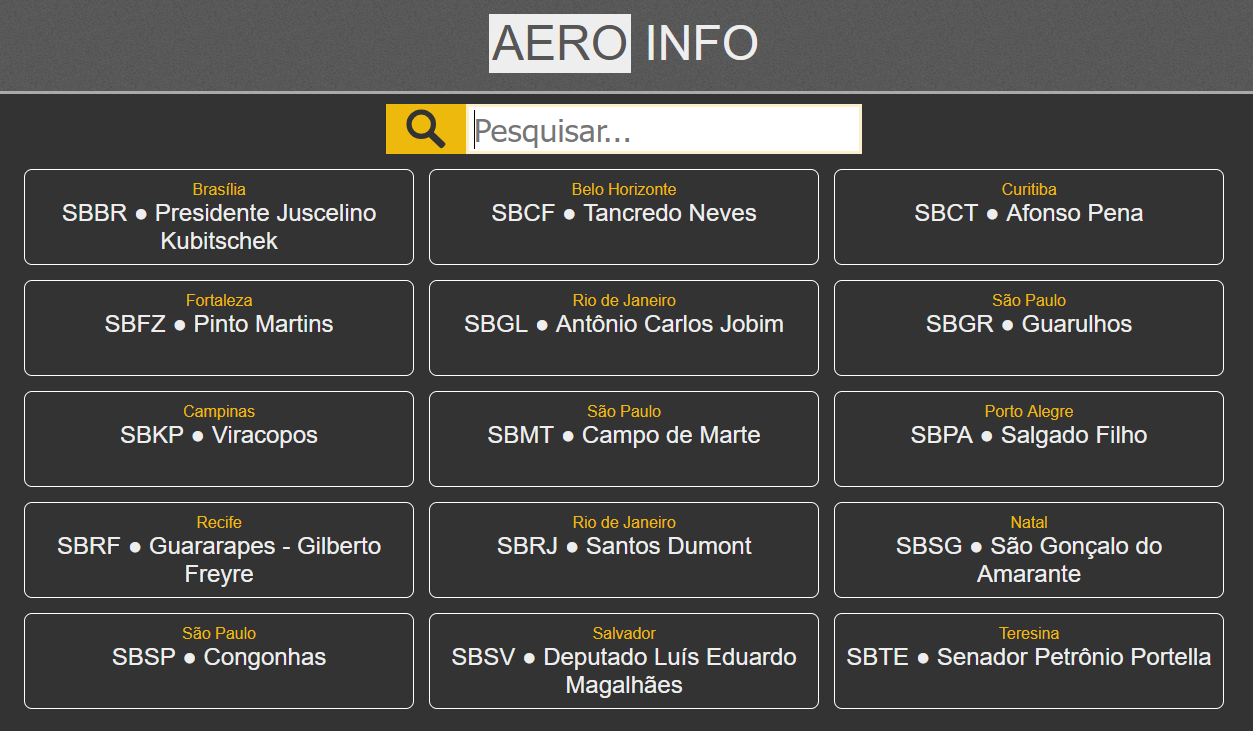
\includegraphics[width=400pt]{img/sel-aeroporto.png}
    \caption{Página Inicial}
    \label{fig:sel-aeroporto}
    \end{center}
\end{figure}

\begin{figure}[ht]
    \begin{center}
    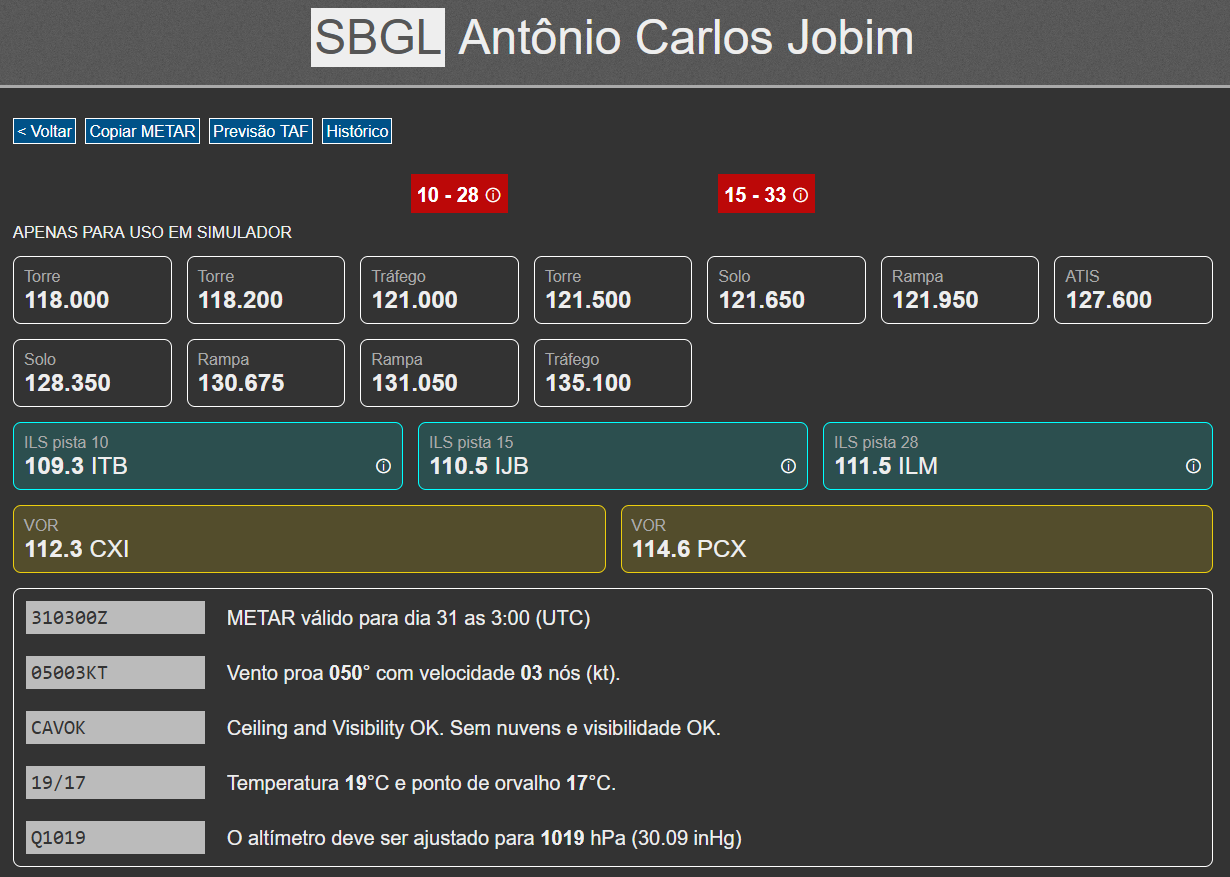
\includegraphics[width=400pt]{img/img-metar.png}
    \caption{Dados do aeroporto e METAR}
    \label{fig:img-metar.png}
    \end{center}
\end{figure}

\begin{figure}[ht]
    \begin{center}
    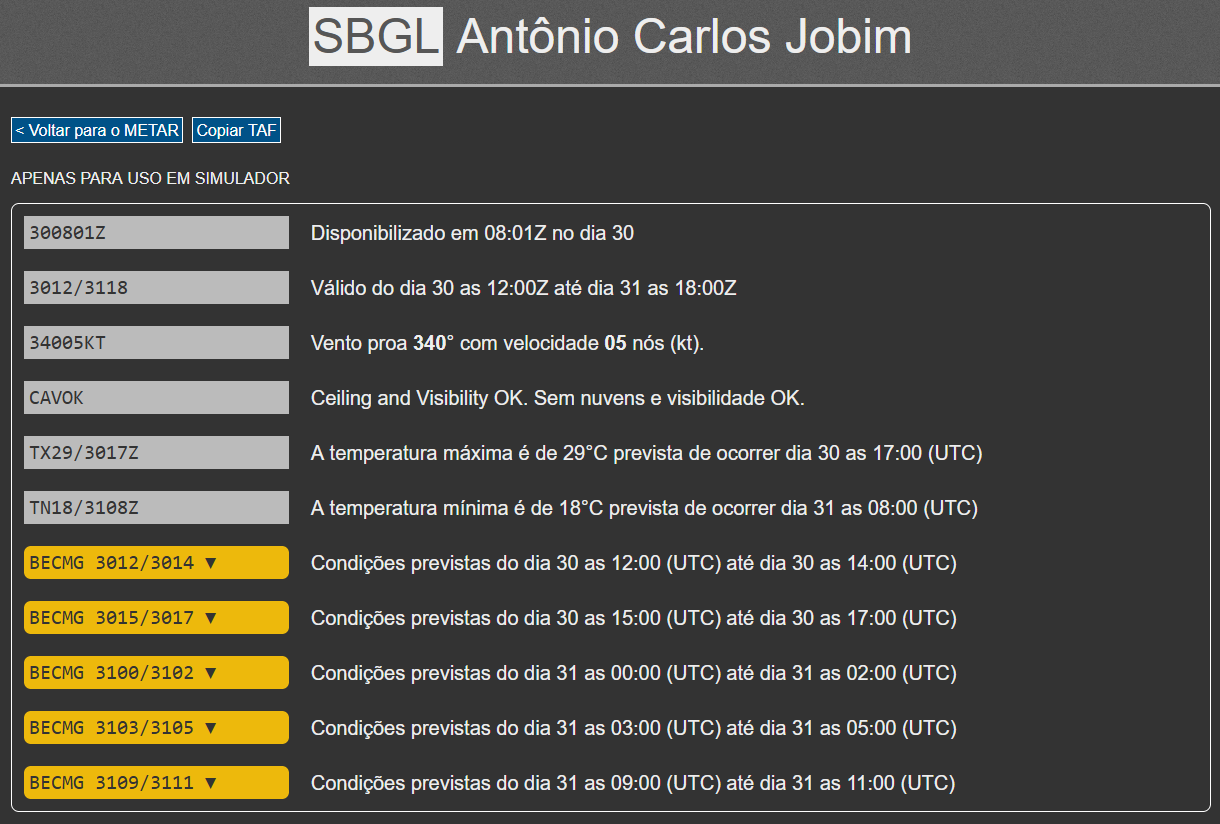
\includegraphics[width=400pt]{img/img-taf.png}
    \caption{TAF}
    \label{fig:img-taf.png}
    \end{center}
\end{figure}

\begin{figure}[ht]
    \begin{center}
    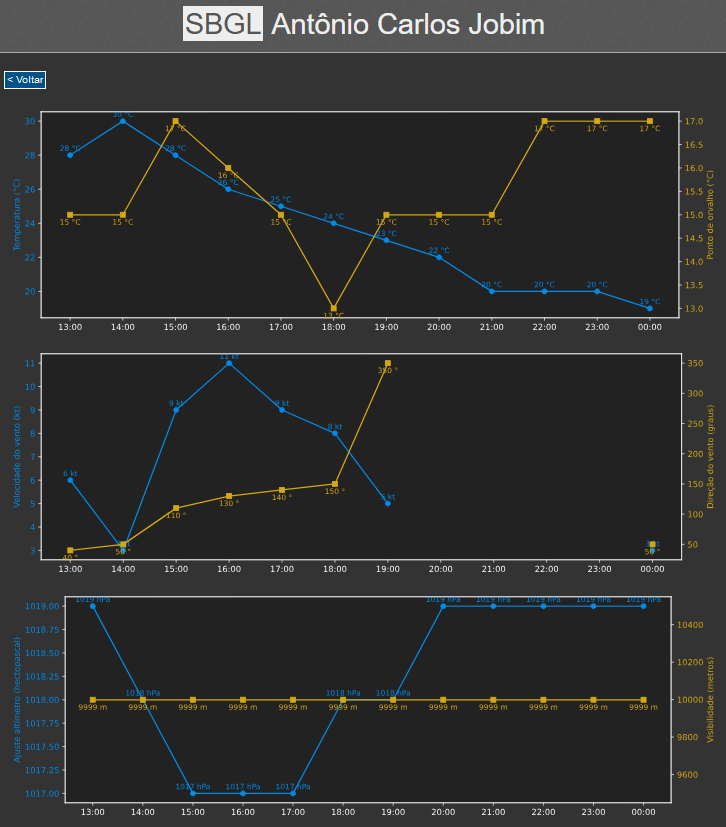
\includegraphics[width=400pt]{img/img-history.png}
    \caption{Plotagem das informações históricas}
    \label{fig:img-history.png}
    \end{center}
\end{figure}

